\section{Network Time Protocol}

\textit{\acrlong{ntp}} \cite{Mills1991} es un protocolo estándar de red 
empleado para la sincronización de relojes en computadores conectados mediante 
redes conmutadas, que fue diseñado por David L. Mills de la Universidad de 
Delaware. Su uso se demostró públicamente por primera vez en 1979, en lo que 
sería una prueba de enlace satelital transatlántico para varios servicios de 
Internet. Posteriormente, en 1985 se implementó NTPv0 para sistemas tipo Unix 
donde la estructura para la cabecera y los cálculos para el tiempo de ida y 
vuelta (o \textit{round-trip time}) y el desfase entre relojes son los que se 
siguen utilizando en la versión actual NTPv4.

Los servidores \gls{ntp} pueden operar en varios modos: \textit{multicast}, 
llamada a procedimiento remoto y simétrico. El modo \textit{multicast} está 
enfocado a redes de área local (\gls{lan}) donde el número de clientes es 
grande y no se necesita de un alto nivel de precisión. En este escenario, uno o 
varios servidores se encuentran continuamente enviando mensajes de difusión 
\gls{ntp} que reciben los clientes que serán los encargados de calcular el 
desfase de su reloj con respecto al del servidor. Los servidores anuncian la 
posibilidad de proveer sincronización pero no aceptan mensajes \gls{ntp} de 
ninguno de los pares.
El segundo modo está pensado para escenarios donde se necesite una gran 
exactitud en la sincronización. Los servidores pueden actuar como cliente 
aceptando la sincronización de otro par (sin proveerla de forma descendente) o 
en modo servidor donde no aceptan ser sincronizados.
Los modos \textit{multicast} y llamada a procedimiento remoto no escalan bien 
en redes grandes de ámbito general como Internet. Para ello, los servidores de 
tiempo deben poder distribuirse de forma dinámica con una topología 
jerarquizada. Para este tipo de modo se emplea la comunicación simétrica donde 
el algoritmo de selección de \gls{ntp} determina el rol de cada uno de los 
servidores en la red.

\subsection{Organización de la red}

La topología de red usada en \gls{ntp} es de tipo jerárquica, donde el índice 
del nivel es un indicativo de la cercanía a la fuente primaria de tiempo. A 
cada nivel de la jerarquía se le denomina estrato. Se comienza a numerar por 0 
y se va sumando 1 por cada nivel de conexión en la jerarquía, es decir, un 
servidor sincronizado a un estrato \textit{n} se encontrará a \textit{n+1} 
saltos de la fuente principal. Este índice indica la distancia a la fuente y no 
necesariamente la calidad del servidor.

\begin{figure}
	\centering
	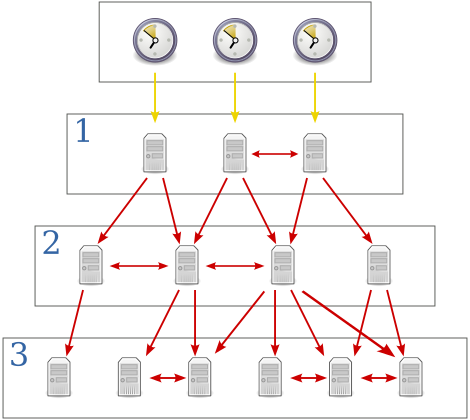
\includegraphics[width=0.7\linewidth]{imagenes/ntp_tree}
	\caption[Esquema de una red de distribución de tiempo usando NTP.]{En este 
	diagrama se 
	muestra una posible red de distribución de tiempo usando NTP. En el estrato 
	0 se hayan las fuentes de reloj de alta estabilidad como GPSDO o relojes 
	atómicos. Estas se conectan directamente a los servidores del estrato 1 que 
	forman los llamados servidores de tiempo primarios. Esta capa provee la 
	hora UTC al resto de los niveles. Como se puede ver se pueden establecer 
	enlaces entre equipos del mismo nivel, además, pueden estar conectados a 
	varios servidores de la capa superior (redundancia). Imagen tomada de 
	\cite{website:imgNTPtree}}
	\label{fig:ntptree}
\end{figure}


El límite superior para un estrato es el 15. Para indicar que un dispositivo no 
está sincronizado se utiliza el valor de estrato 16. El algoritmo \gls{ntp} 
está diseñado para construir una topología con los caminos más cortos hacía los 
servidores del estrato 1 (haciendo uso del algoritmo Bellman-Ford) lo que 
minimiza el tiempo de ida y vuelta acumulado entre los servidores de estrato 1 
y los clientes. A continuación se describen brevemente los estratos más 
relevantes:

\begin{itemize}
	\item \textbf{Estrato 0} \\ A este nivel se encuentran las fuentes de 
	tiempo de alta precisión, entre las que cabe destacar los relojes atómicos 
	o los osciladores disciplinados por GPS (\acrshort{gpsdo}). Generan una 
	señal de un pulso por segundo (\acrshort{pps}) que permite disciplinar el 
	oscilador interno del servidor conectado a la fuente de nivel 0.
	
	\item \textbf{Estrato 1} \\ Lo forman los servidores cuyos relojes se 
	disciplinan directamente con la señal recibida de una fuente de nivel 0 
	logrando una sincronización en torno a unos pocos microsegundos. Además 
	pueden conectarse con otros del mismo nivel para tareas de comprobación de 
	errores o para redundancia.
	
	\item \textbf{Estrato 2 (en adelante)} \\ Los dispositivos de cada estrato 
	se 
	sincronizan con el estrato anterior, pudiendo hacerlo con varios servidores 
	a la vez, y además pueden hacerlo con otros computadores del mismo nivel a 
	fin de mejorar la calidad del servicio.
\end{itemize}

\subsection{Algoritmo}

La figura \ref{fig:ntptree} muestra un esquema de organización típico para una 
red de distribución de tiempo usando \gls{ntp}. Para realizar el cálculo del 
desfase del reloj cliente con respecto al servidor, se emplean una serie de 
paquetes con marcas de tiempo (\textit{timestamps}). El cliente debe iniciar el 
proceso realizando una petición al servidor como muestra la figura 
\ref{fig:ntpts}. El servidor recibe el paquete y lo sella en el instante $T_i$. 
Para realizar los cálculos se emplean siempre las 4 marcas más recientes. Con 
ello se puede realizar el cálculo del tiempo de ida y vuelta ($\delta_i$), y el 
desfase del reloj ($theta_i$) del cliente con respecto al del sevidor en el 
instante de tiempo $T_i$:

\begin{equation}\label{ntprtt}
	\delta_i = (T_{i-2}-T_{i-3}) - (T_{i-1}-T_{i})
\end{equation}\label{ntpoffset}
\begin{equation}
	\theta_i = \frac{(T_{i-2}-T_{i-3}) + (T_{i-1}-T_{i})} {2}
\end{equation}

Hay que tener en cuenta que el servidor no tiene por qué contestar a las 
peticiones del cliente de forma inmediata. El proceso encargado de la gestión 
del servicio \gls{ntp} puede ser interrumpido por otra tarea con más prioridad, 
lo que hace que el tratamiento de las marcas de tiempo no sea determinista.

\begin{figure}
	\centering
	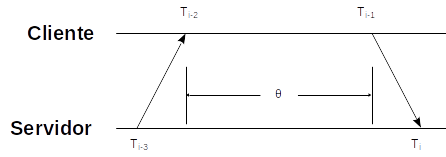
\includegraphics[width=0.7\linewidth]{imagenes/ntp_ts}
	\caption[Cálculo del desfase entre cliente y servidor]{La figura muestra un 
	intercambio de paquetes con marcas de tiempo entre cliente y servidor. Para 
	calcular el tiempo de ida y vuelta se utilizan 4 marcas de tiempo.}
	\label{fig:ntpts}
\end{figure}

\subsection{Rendimiento}

Al ser \gls{ntp} un protocolo que se implementa completamente en 
\textit{software}, no se consigue una gestión determinista para el cálculo del 
desfase entre las dos entidades que se sincronizan. Ello conlleva una 
limitación severa a la exactitud alcanzable mediante el uso de este protocolo 
\incomment{Mejorar esa frase}. Aunque este hecho podría ser tratado mediante el 
uso de sistemas operativos de tiempo real o técnicas que consigan reducir la 
latencia con la que el proceso encargado de la gestión del protocolo \gls{ntp} 
es ejecutado, existe otro factor de diseño que tiene incluso más peso en la 
precisión alcanzable por éste: la asunción de igualdad entre los caminos de ida 
y vuelta para los paquetes enviados por la red de comunicación. En \gls{ntp} se 
considera que el camino de transmisión de los paquetes es simétrico al camino 
de recepción, lo cual es bastante improbable en redes conmutadas con varios 
saltos y múltiples caminos como es el caso de Internet. Todo ello conlleva que 
la exactitud que alcanza este protocolo de forma general, sincronizando dos 
equipos, se sitúe en el orden de los milisegundos llegando a decenas de 
microsegundos en condiciones controladas.